\documentclass[12pt]{article}

\usepackage[english]{babel}
\usepackage{geometry}
\usepackage{graphicx}
\usepackage{float}
\usepackage{extsizes}
\usepackage{blindtext}
\usepackage{wrapfig}
\usepackage[format=plain, textfont=sl, font=footnotesize]{caption}
\usepackage{hyperref}

\geometry{
 a4paper,
 total={170mm,257mm},
 left=20mm,
 top=20mm,
 }
\graphicspath{ {../res/} }
\hypersetup{
    colorlinks = false,
    pdftitle = {Dwarf Guide},
    pdfpagemode=FullScreen,
}
\captionsetup[figure]{labelformat=empty}

\title{Dwarf Guide}
\author{h4nto}

\begin{document}

% FIRST PAGE:

\topskip0pt
\begin{center}
    \vspace*{\fill}
    \Huge\textbf{Dwarf Guide} \\
    \begin{figure}[h]
        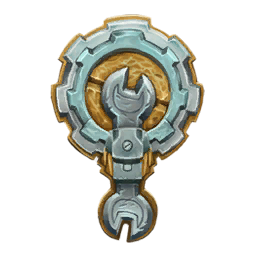
\includegraphics{dwarf.png}
        \centering
    \end{figure}
    \vspace*{\fill}
    \normalsize{A detailed Steam Mechanicus guide to help beginners,\\mid game and end game players and pvp players.} \\
    \vspace*{\fill}
    \Large\textsl{Written by h4nto} \\
    \Large\textsl{h4nto\#6969}
    \vspace*{\fill}
\end{center}

\newpage

% INDEX:

\tableofcontents

\newpage

% BEGINNERS:

\section{Beginners}

\subsection{Wisdom}
Talking about Wisdom, the first things to focus on are Attack Speed (put there points until you reach 4.00 Attack Speed, so you will get the damage buff in map) and most of all Critical (to max 80/80 as soon as possible). \\
After that you can start using your points on what you think you need at that moment. \\
Generally it's defensive stats such as HP, Armor and Resistances or eventually some Steam if you feel you run out of resources too quickly.

\subsection{Group Tree}
In the Group Aura section you should first of all upgrade the Racing the Clock Talent (which grants some extra Cooldown Reduction). \\
After that you want to start upgrading the Wisdom, Realm Fragments and Andermants Talent (in this order). \\
In the end you will max out also the Anxiety Shards Talent and the Upgraded Spheres one in the Group Aura section (when group level maxed you can put the remaining 4 points on Light Resistance).

\subsection{Gems}
Talking about Gems, as always Critical is the most important thing, try to have a balanced build but most of all work to get the 4.00 Attack Speed and upgrade your Critical gems as much as possible. \\
Other Gems to equip are Movement Speed, Damage and HP at last.

\subsection{Runes}
Talking about Runes, first of all you should work on your Wisdom and Materi runes (upgrade them as much as possible because they will allow you to level up your Wisdom way faster and also get faster the Materi to buy Infernal Passages). \\
After them again focus first on Attack Speed and Critical. Then go for HP, Damage and Movement Speed but don't throw away Steam and Steam Regeneration ones, equip them and upgrade them later. \\
Another Rune that is particularly good is Realm Fragment Talent Rune (you will need to max that in order to join groups for Realm Fragments farm) together with Wisdom and Andermants Talent Runes. \\
Every other kind of Rune you can melt for now.

\subsection{Jewels}

\subsection{Items}

% 1 HAND FIRE BUILD:

\subsection{1 Hand Fire Build}
\subsubsection{Build}
\subsubsection{Skilltree}
\subsubsection{Gameplay}

\newpage

% MID GAME:

\section{Mid Game}

\subsection{Wisdom}
Talking about Wisdom, you should have reached here a good amount of Wisdom so you can manage and balance pretty well your point. \\
You should have maxed Critical, the needed Attack Speed in order to have at least 4.00, Cooldown Reduction in case you are playing a 2 hand build (which is one of the main reasons why you switch to a 2 hand build) and Damage.

\begin{wrapfigure}{r}{0.47\linewidth}
    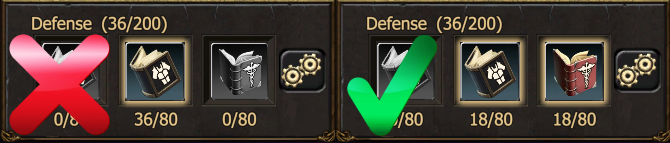
\includegraphics[width=8cm]{wisdom/wisdom_example.png}
    \caption{Balancing stats example with 36 points.}
    \centering
\end{wrapfigure}
You should also have balanced defensive stats (HP which i'd suggest aiming to have at least 1m, Resistance and Armor). For what concerns Resistance and Armor always level them up together like 40/80 and 40/80, and not one at a time like 80/80 and 1/80. \\
And last but not least if you feel like needing some extra Steam for your skills you can put there some points. \\
A Talent that will really help you a lot is the Close to Turret one in the Combat section (300 Wisdom points for extra Cooldown Reduction when inside the Turrets range). I suggest going for that talent when you have approximately around 1k total Wisdom points so you can still manage to have enough points in the other sections. \\
Another Talent that could help you a lot especially when doing Bloodchests is the Peddler (the portable shop) in Prosperity section.

\subsection{Gems}
\subsection{Runes}
\subsection{Jewels}
\subsection{Items}
% 1 HAND LIGHT BUILD:
\subsection{1 Hand Light Build}
\subsubsection{Build}
\subsubsection{Skilltree}
\subsubsection{Gameplay}
% 2 HAND LIGHT BUILD:
\subsection{2 Hand Light Build}
\subsubsection{Build}
% 2 HAND FIRE BUILD:
\subsection{2 Hand Fire Build}
\subsubsection{Build}

\newpage

% END GAME:

\section{End Game}
\subsection{Wisdom}
\subsection{Gems}
\subsection{Runes}
\subsection{Jewels}
\subsection{Items}
\subsection{Build}
% OPTIMAL BUILD:
\subsection{Optimal Build}
\subsubsection{Build}
\subsubsection{Skilltree}
\subsubsection{Gameplay}

\newpage

% PVP:

\section{PvP}
\subsection{PvP Tree}
\subsection{Gems}
\subsection{Items}
% 1 HAND POISON BUILD:
\subsection{1 Hand Poison Build}
\subsubsection{Build}
\subsubsection{Skilltree}
\subsubsection{Gameplay}

\subsection{Swerfield}

% GENERAL TIPS:

\section{General Tips}

\end{document}